% !TeX TXS-program:compile = txs:///pdflatex/[--shell-escape]
% Le truc au-dessus pour avoir l'option shell-escape qui permet de faire du minted.
\documentclass[12pt]{article}

% Affichage ou non des reponses aux questions & exercices
\newif\ifDispRep
\DispReptrue  % Show the text
%\DispRepfalse % Hide the text

% Version du document
\newcommand{\versiondoc}{v0.2}

% Incorporation tous éléments de préambule communs à tous mes cours
\usepackage{../../../CoursLFC}

% Eléments de l'en-tête et de la page de garde spécifiques à ce doc
\newcommand{\classe}{1\textsuperscript{ère} NSI}
\newcommand{\themecours}{Thème 4: Représentation des données}
\newcommand{\datedoc}{novembre 2023}

% Page de garde mise en page
\title
	{\vspace{3cm}
		{\Large
		\textit
			{
				\classe\hspace{0.1cm}
				\textemdash\
				\hspace{0.1cm}
				\themecours
			}
			
		\vspace{1cm}
		\huge{Types \& Valeurs de base} }
		 
		\vspace{1cm}
	}
\author{\etablissement}
\date{
	\auteur,
	\datedoc,
	\footnotesize{\textit{\versiondoc}} 
	\vspace{6cm}
	}

% Header & Footer
\lfoot{\etabshort}
\cfoot{\thepage}
\rfoot{\classe, \anneescol}
\renewcommand{\footrulewidth}{0.2pt}
\lhead{}
\chead{}
\rhead{}
\renewcommand{\headrulewidth}{0pt}

\begin{document}
	
	\maketitle
	% pas de footer sur la première page
	\thispagestyle{empty}
		
	\section*{}
		{\noindent
		\resumecours
		}
		
	\pagebreak	
	\tableofcontents
	
	\pagebreak
	
	% Début du contenu du document
	\section{Point d'étape -- où est-on / où va-t-on?}
	\subsection{Ce qu'on a couvert jusqu'à présent}
	
	\begin{itemize}
		\item Rudiments de l'architecture physique d'un ordinateur - le modèle de Von Neumann.
		\item Mise en jambes sur de l'écriture de code: réalisation d'une page Web en HTML.
		\item Et surtout: introduction à Python, et plus spécifiquement:
		\begin{itemize}
			\item Ce qu'on appelle ses "constructions élémentaires" -- variables, fonctions, conditions \& embranchements, boucles...
			\item Les types et valeurs de base: entiers (naturels et relatifs), flottants (réels), chaînes de caractères et booléens (qu'on n'a que brièvement abordés pour l'instant).
			\item Un type dit "construit" -- les listes.
		\end{itemize}
	\end{itemize}
	
	\subsection{Ce dont on va parler dans ce nouveau chapitre}
	On va prendre un pas de recul par rapport au chapitre sur Python -- et se demander comment les données qu'on manipule sont stockés dans l'ordinateur. Après tout, on sait que celui-ci ne manipule que des 0 et des 1; donc comment peut-il stocker \texttt{12} ou \texttt{$\pi$} ou \texttt{"Bonjour!!"}? 
	
	C'est à ces questions qu'on va répondre en étudiant comment différents types de données sont \textbf{\textit{représentés}} dans la mémoire de l'ordinateur
	
	Spécifiquement, on va aborder les points suivants:
	\begin{itemize}
		\item Représentation des entiers naturels;
		\item Représentation des entiers relatifs;
		\item Représentation des nombres réels ("nombres flottants");
		\item Représentation et codage du texte;
		\item Représentation des booléens -- opérateurs booléens, logique boolénne -- ce qui nous amènera à:
		\item Circuits logiques élémentaires.
	\end{itemize}
	
	\subsection{Comment on va procéder}
	On passe ici dans un mode beaucoup plus théorique:
	\begin{itemize}
		\item On ne cherche plus à \textit{faire faire} quelque chose à l'ordinateur (comme en programmation);
		\item On cherche plutôt à comprendre \textit{comment l'ordinateur lui-même fonctionne}.
		\item On va s'intéresser à des aspects beaucoup plus mathématiques de l'informatique.
	\end{itemize}
	\vspace{\baselineskip}
	On va donc devoir travailler différemment du chapitre sur l'introduction à Python:
	 \begin{itemize}
	 	\item \textbf{Prise de notes essentielle};
	 	\item Plusieurs exercices sur papier qu'on fera en classe et dont il sera très important que vous gardiez une trace;
	 	\item $\underline{\textbf{Attention:}}$ régulièrement je vous demanderai de terminer à la maison les exercices commencés en classe -- il faudra donc en avoir pris suffisamment de notes!
	 	\item Quand même, quelques applications / exercices sur machine.
	 \end{itemize}
	 
	 \pagebreak
	 
	 \section{Bases de numération \& Représentation des entiers naturels}
	 
	 
	 \subsection{La base 10}
	 
	 % Questions rhétoriques et réponses escamottables associées
	 Quelques questions "simples" pour commencer...
	 \MaQuestion{Que veut dire "\texttt{2754}"}
% MCO: NE MARCHE QUE SI PAS INDENTE DU TOUT, bordel...	 
\begin{MaReponse}
	Implicitement, c'est une somme de puissances de 10: \[ 2 \cdot 10^3 + 7 \cdot 10^2 + 5 \cdot 10^1 + 4 \cdot 10^0 \]
\end{MaReponse}
	 
	 \MaQuestion{Autrement dit: comment fonctionne la base 10}
\begin{MaReponse}
	Plus généralement, c'est donc une somme de puissances de 10 lue de droite à gauche (puisque si l'on ne regarde que le premier chiffre d'un nombre on ne peut pas savoir à quelle puissance il correspond). Cela revient à dire qu'un nombre \texttt{ABCDEF} écrit en base 10 se lit: \[ F \cdot 10^0 + E \cdot 10^1 + D \cdot 10^2 + C \cdot 10^3 + B \cdot 10^4 + A \cdot 10^5\]
\end{MaReponse}

	 \MaQuestion{Pourquoi la base 10 s'appelle-t-elle la base 10}
\begin{MaReponse}
	Tout simplement parce qu'elle permet d'écrire la totalité de tous les entiers naturels en n'utilisant que 10 symboles -- les 10 chiffres arabes: 1, 2, 3, 4, 5, 6, 7, 8, 9 -- et le plus important de tous: 0.
\end{MaReponse}

	 \MaQuestion{Pourquoi utilise-t-on la base 10}
\begin{MaReponse}
	Deux remarques pour commencer: d'abord, on n'utilse pas que la base 10 -- pensez par exemple aux oeufs qu'on compte encore aujourd'hui par douzaines; ensuite, il n'y a pas de réponse certaine à cette question. La plus intuitive est que cela correspond à nos doigts -- on en a 10, donc quand on les a tous "utilisés" on repart du premier, comme on fait avec les chiffres à l'écrit.
\end{MaReponse}

	 \MaQuestion{Comment s'appellent les symboles utilisés pour écrire des nombres en base 10}
\begin{MaReponse}
	Ca a été dit plus haut -- ce sont les chiffres, inventés en Inde, puis parvenus en Europe par le monde arabe (d'où leur nom) aux environs du \textsc{x}\ieme ~siècle.
\end{MaReponse}
	 
	 \pagebreak
	 \subsection{Et en base \sout{Shadok} 4, par exemple?}
	 
	\begin{wrapfigure}{r}{0.\textwidth}
		
\includegraphics[scale=0.2]{001_Shadok.png}
	\end{wrapfigure}
	 Les Shadoks, c'est un dessin animé absurde français des années 60 -- l'histoire d'oiseaux aux ailes ridiculement petites habitant sur une autre planète qui veulent conquérir l'univers; pour ça ils ont besoin de la science. Donc de pouvoir compter. Leur problème? Leur langue ne contient en tout et pour tout que quatre mots: \textbf{\texttt{GA}}, \textbf{\texttt{BU}}, \textbf{\texttt{ZO}}, et \textbf{\texttt{MEU}}....
	
	 Alors comment faire....?
	 
	\textbf{ \href{https://www.youtube.com/watch?v=9bNZjP1LsNA}{Allons voir la solution qu'ils ont retenue...}}
	
	\vspace{\baselineskip}
	
	Récapitulons:
	\begin{tabular}{|c|c|c|}
			\hline
			\textbf{Mot} & \textbf{Symbole} & \textbf{Quantité} \\
			\hline
			GA & \raisebox{-0.4\height}{
\includegraphics[width=5mm]{002_Ga.png}} & -  \\
			\hline
			BU & \raisebox{-0.4\height}{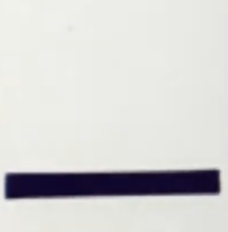
\includegraphics[width=5mm]{003_Bu.png}} & I \\
			\hline
			ZO & \raisebox{-0.4\height}{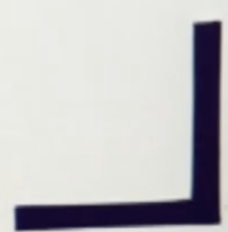
\includegraphics[width=5mm]{004_Zo.png}} & I I \\
			\hline
			MEU & \raisebox{-0.4\height}{
\includegraphics[width=5mm]{005_Meu.png}} & I I I \\
			\hline
	\end{tabular}
	
	\vspace{\baselineskip}
		
	\begin{MonExo}[conversions d'une base à une autre]
		Convertissez en base 10 les quantités exprimées en base Shadok suivantes:
		\begin{alphenum}
			\item Zo
			\item Bu Zo
			\item Meu Meu
			\item Zo Ga
			\item Meu Zo Ga
		\end{alphenum}
		\textit{Souvenez-vous: on compte, de droite à gauche, des Shadoks, puis des "poubelles" 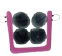
\includegraphics[width=10mm]{007_Poubelle.png} de quatre Shadoks, des "grandes poubelles" 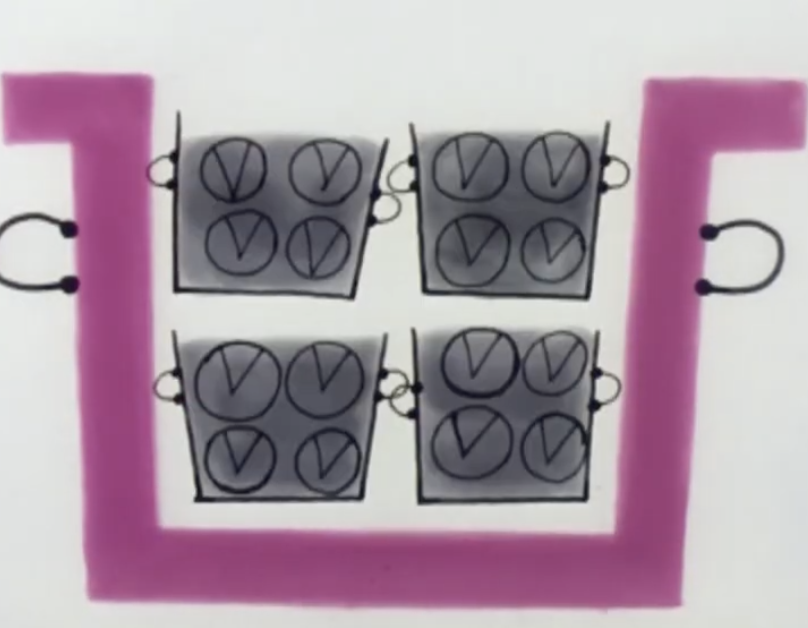
\includegraphics[width=10mm]{008_GdePoubelle.png}qui contiennent chacune quatre poubelles, etc... }
	\end{MonExo}
	
	\begin{MaReponse}
		Prenons d'entrée de jeu ici l'habitude d'aborder les nombres de droite à gauche -- donc en commençant par les Shadoks, puis les poubelles, puis les grandes poubelles, etc...
		\begin{alphenum}
			\item Zo = 2 -- c'est écrit dans le tableau.
			\item Bu Zo -- on a zo, donc deux, Shadoks (chiffre de droite); et on a bu, donc une, poubelle qui contient 4 Shadoks. Donc Bu Zo = $2\times1 + 1\times4 = 6$.
			\item Meu Meu -- même raisonnement: meu Shadoks, donc 3, et meu poubelles, donc $3\times4$; donc Meu Meu $= 3\times1 + 3\times4 = 15$.
			\item Zo Ga -- même chose, sauf que cette fois il y a ga, donc zéro, Shadoks a droite: Zo Ga $= 0\times1 + 2\times4$
			\item Meu Zo Ga -- toujours la même démarche, sauf qu'on a cette fois un chiffre de plus, donc des grandes poubelles contenant chacune 4 poubelles de 4:  \[ 0 \times 1 + 2 \times 4 + 3 \times 16 = 56 \]
		\end{alphenum}
	\end{MaReponse}
	
	\begin{MonExo}[et maintenant sauvons le pauvre Professeur Shadoko...]
		Convertissez le nombre mystère 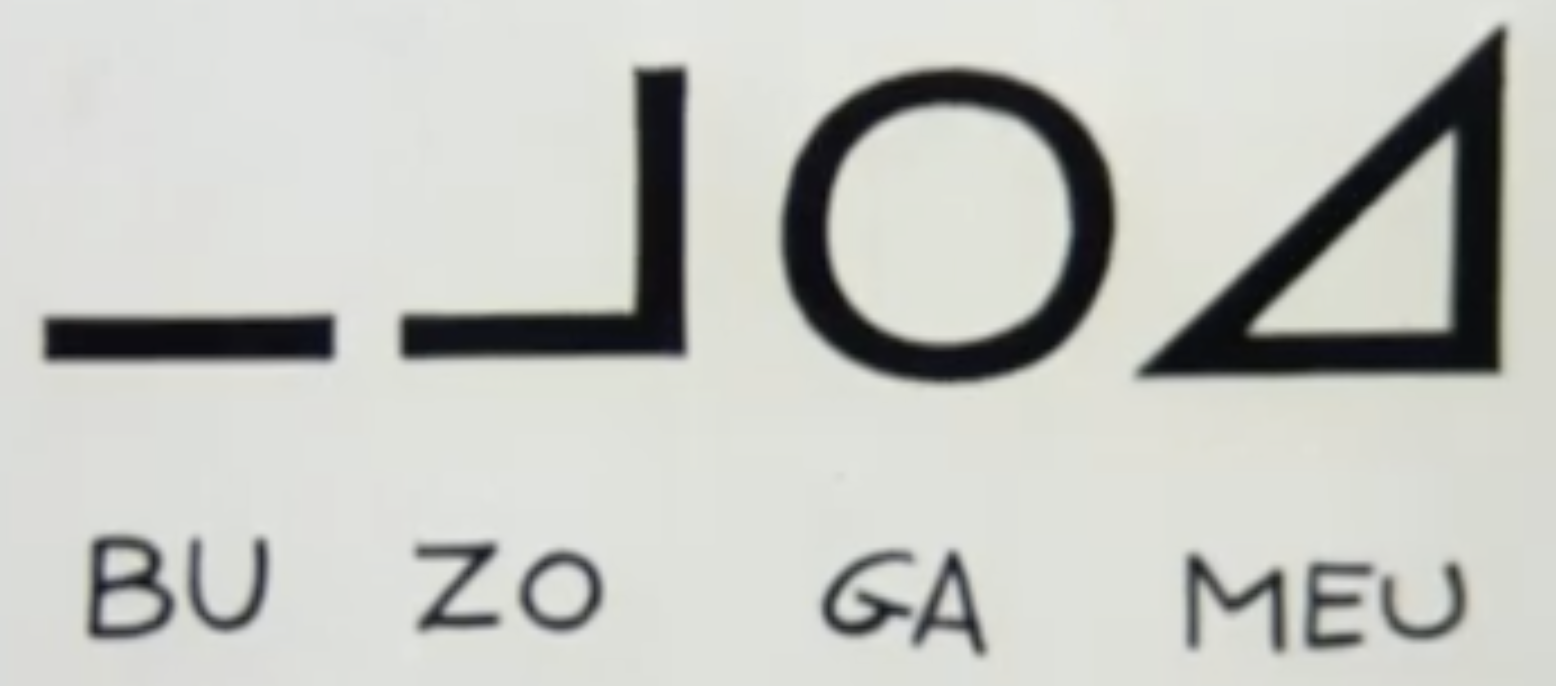
\includegraphics[width=30mm]{006_BuZoGaMeu.png} en français.
	\end{MonExo}
	
	\begin{MaReponse}
		Même chose que dans l'exercice précédent, sauf qu'on introduit ici un quatrième chiffre -- les "super poubelles" qui contiennent 4 grandes poubelles, qui contiennent 4 poubelles, qui contiennent 4 Shadoks -- donc $4\times4\times4$; il serait peut-être temps de parler en puissances de 4, non?
		\[ Meu \times 4^0 + Ga \times 4^1 + Zo \times 4^2 + Bu \times 4^3\] 
		\[= 3 \times 1 + 0 \times 4 + 2 \times 16 + 1 \times 64 = 99\]
	\end{MaReponse}
	
	\begin{MonExo}[plus généralement...]
		Proposez une méthode pour convertir un nombre Shadok dans notre système d'écriture courant.
	\end{MonExo}
	
	\begin{MaReponse}
		On ne propose ici qu'une généralisation de ce qu'on a fait jusqu'à present: partir du chiffre de droite, le multiplier par $4^0$, soit $1$; passer au chiffre suivant, le multiplier par $4^1$, soit $4$, et l'ajouter au précédent; continuer ainsi vers la gauche en augmentant à chaque fois les puissances de 4 et en ajoutant au precedent jusqu'à atteindre le chiffre le plus à gauche.

		En pseudo-code, on pourrait écrire:
		
		\begin{algorithmic}[1]
			\Require{$nbB4 \in \mathds{N}$, exprimé en base 4}
			\Ensure{$resB10 \in \mathds{N}$, exprimé en base 10}
			\Function{ConvertirBase4enBase10}{nbB4}
			\State resB10 $\leftarrow$ 0
			\State puiss $\leftarrow$ 0
			\ForAll{chiffre de nbB4}

			\Comment{Parcours des chiffres \textbf{de droite à gauche}}
			
			\State resB10 $\leftarrow$ resB10 + chiffre$\times 4^{puiss}$
			\State puiss $\leftarrow$ puiss + 1
			\EndFor
			\State\Return{resB10}
			\EndFunction
		\end{algorithmic}
	\end{MaReponse}
	
		
	Bon -- abandonnons le vocabulaire Shadok à présent et revenons au cours: on parle évidemment ici d'une \textbf{base 4} et notre méthode générale peut s'écrire sous la forme d'une suite de puissances de 4.
	
	Pour un nombre N noté en base 4 \( a_4 \)\( a_3 \)\( a_2 \)\( a_1 \)\( a_0 \), par exemple, on le convertira par la formule:
	
	\[ N = a_0 \cdot 4^0 + a_1 \cdot 4^1 + a_2 \cdot 4^2 + a_3 \cdot 4^3 + a_4 \cdot 4^4\]
	
	Ou encore:
	
	\[ N = a_0 \cdot 1 + a_1 \cdot 4 + a_2 \cdot 16 + a_3 \cdot 64 + a_4 \cdot 256\]
	
	Et plus généralement, pour un nombre N noté en base 4 \( a_k \)\( a_{k-1} \)(...)\( a_2 \)\( a_1 \)\( a_0 \), on aura:
	
	\[ N = \underbrace{a_0 \cdot 4^0 + a_1 \cdot 4^1 + a_2 \cdot 4^2 + (...) + a_{k-1} \cdot 4^{k-1} + a_k \cdot 4^k}_{\text{(k+1)\ éléments, de 0 à k}}\]
	
	ce qui s'écrit aussi:
	
	\[ N = \sum_{i=0}^{k} a_i \cdot 4^i \]
	
	Donc si on remplace Ga, Bu, Zo, et Meu par les chiffres arabes correspondants (0, 1, 2, 3), on pourra dire que le nombre 132 en base 4 vaut 46 en base 10:
	
	\[ 2 \cdot 4^0 + 3 \cdot 4^1 + 1 \cdot 4^2  = 2 \cdot 1 + 3 \cdot 4 + 2 \cdot 16 = 46\]
	
	Pour exprimer cela simplement, on va placer la base d'expression du nombre en indice de celui-ci et écrire: $132_4$ = $46_{10}$
	
	\begin{MonExo}[et dans l'autre sens?]
		Convertissez en base 4 (ou en Shadok, comme vous préférez) les nombres écrits en base 10 suivants:
		\begin{alphenum}
			\item $16_{10}$ =
			\item $17_{10}$ =
			\item $64_{10}$ =
			\item $65_{10}$ =
			\item $11_{10}$ =
			\item $25_{10}$ =
			\item $57_{10}$ =
			\item $675_{10}$ =
		\end{alphenum}
	\end{MonExo}
	
	\begin{MaReponse}
		On reprend à partir de maintenant les chiffres arabes pour noter nos nombres -- ceux de 0 à 9 quand on est en base 10, et ceux de 0 à 3 en base 4 (qui remplacent donc Ga a Meu en base Shadok).
		
		On a remarqué en classe que les 4 premiers exemples de cet exercice sont des valeurs \textbf{très} proches de puissances de 4 -- et ce n'est évidemment pas un hasard:
		\begin{tabbing}
			$16_{10}$ \==  $(4^{2})_{10}$ \\
			\>= $(1 \times 4^{2} + 0 \times 4^{1} + 0 \times 4^{0})_{10}$ \\
			\>= $(100)_{4}$
			\\ \\
			$17_{10}$ \==  $(16 + 1)_{10}$ \\
			\>=  $(4^{2} + 1)_{10}$ \\
			\>= $(1 \times 4^{2} + 0 \times 4^{1} + 1 \times 4^{0})_{10}$ \\
			\>= $(101)_{4}$
		\end{tabbing}
		Et de la même manière, on obtient pour les deux suivants:
		
		$64_{10}$ =  $(4^{3})_{10}$ =  $1000_{4}$
		
		$65_{10}$ =  $(4^{3} + 1)_{10}$ =  $1001_{4}$

		Pour les questions e) à h), on applique rigoureusement la méthode que l'on va decrire a l'exercice suivant et on obtient:
		\begin{enumerate}[label=\alph*.,start=5]
			\item $11_{10}$ = $23_4$
			\item $25_{10}$ = $121_4$
			\item $57_{10}$ = $321_4$
			\item $675_{10}$ = $22203_4$
		\end{enumerate}
	\end{MaReponse}
	
	\begin{MonExo}[ça commence à devenir un poil compliqué...]
		Proposez cette fois une méthode pour convertir un nombre de base 10 en base 4 (ou Shadok).
	\end{MonExo}
	
	% ICI IL FAUT NOTER LES DEUX METHODES
	\begin{MaReponse}
		Pour convertir le nombre $N_{10}$ en base 4, on va procéder de la manière qui suit:
		\begin{enumerate}
			\item On cherche d'abord la première puissance $k$ de 4 qui soit strictement supérieure à $N_{10}$
			\item On dresse un tableau avec les premières puissances de 4, de $4^{k-1}$ à $4^0$.
			\item On effectue une division euclidienne de $N_{10}$ par $4^{k-1}$ et on note le quotient de cette division dans la case $4^{k-1}$ du tableau.
			\item On soustrait $4^{k-1l}$ de $N_{10}$a plus grande puissance de 2 qui est inférieure au nombre à convertir.
			\item On prend le reste de cette division et on répète ces étapes jusqu'à arriver à un quotient inférieur à 4.
		\end{enumerate}

		Exemple, pour convertir le nombre $710_{10}$:
		
		$256 \le 710 < 1024$

		Donc: $4^4 \le 710 < 4^5$
		
		Donc on dresse le tableau des puissances de 4 de l'exposant 4 à l'exposant 0:
		
		\[
		\begin{array}{|c|c|c|c|c|c|c|}
		\hline
		4^4 & 4^3 & 4^2 & 4^1 & 4^0 \\
		\hline
		256 & 64 & 16 & 4 & 1 \\
		\hline
		2 & 3 & 0 & 1 & 2 \\
		\hline
		\end{array}
		\]
		
		\[
		\begin{array}{llll}
		710 // 256 &= 2 &\quad \text{(reste = } 198 \text{)} &\quad \text{(on place un "2" dans la case \(256\))} \\
		198 // 64 &= 3 &\quad \text{(reste = } 6 \text{)} &\quad \text{(on place un "3" dans la case \(64\))} \\
		6 // 4 &= 1 &\quad \text{(reste = } 2 \text{)} &\quad \text{(on place un "1" dans la case \(4\))} \\
		2 < 4 &&&\quad \text{(on place un "2" dans la case \(1\))} \\
		\text{Fin} & \\
		\end{array}
		\]
		
		Le nombre \(710_{10}\) se convertit donc en \(23012_{4}\).
		
		%\hl{\textbf{A REDIGER}}
	\end{MaReponse}
		
	\subsection{La base 2 -- ou "numération binaire"}
	
	\subsubsection*{Quel rapport avec l'informatique?}
	
	Imaginons un interrupteur électrique: il peut être soit en position \textit{ON}, soit en position \textit{OFF}. En informatique, le "coeur" d'un ordinateur est composé de millions voire de milliards de petits "interrupteurs" appelés \textbf{\textit{transistors}}.
	
	Un transistor permet à un courant électrique de passer (état "allumé" -- que l'on va appeler "1") ou non (état "éteint" ou "0"). C’est cette simplicité qui rend les transistors fiables et efficaces pour construire des circuits électroniques complexes comme ceux que l'on trouve dans les processeurs d’ordinateur. Ainsi, la mémoire de l’ordinateur utilise des transistors pour stocker des informations sous forme de 1 et de 0 selon l'état des transistors qui la composent .
	
	Toute information, de quelque nature qu'elle soit, doit être convertie en 1 et en 0 pour être manipulée par un ordinateur.
	
	Donc en base 2.
	
	Donc en binaire.
	
	\subsubsection*{Conversions de et vers la base 2}
	
	C'est à présent que les Shadoks vont venir à notre secours: parce que le principe en base 2 est rigoureusement le même qu'en base 4 -- sauf qu'au lieu d'utiliser 4 symboles (0, 1, 2, et 3), on n'en utilise que 2 (0 et 1) et qu'au lieu de manipuler des puissances de 4, on manipule des puissances de 2. Pour un nombre N noté en base 2 \( a_k \)\( a_{k-1} \)(...)\( a_2 \)\( a_1 \)\( a_0 \), on aura:
	\[ N = \underbrace{a_0 \cdot 2^0 + a_1 \cdot 2^1 + a_2 \cdot 2^2 + (...) + a_{k-1} \cdot 2^{k-1} + a_k \cdot 2^k}_{\text{(k+1)\ éléments, de 0 à k}}\]
	
	ce qui s'écrit aussi:
	
	\[ N = \sum_{i=0}^{k} a_i \cdot 2^i \]
	
	\begin{MonAmp}{Conseil}
		Vous allez vite vous rendre compte que pour ce chapitre et pour la matière NSI en général on gagne beaucoup de temps en connaissant les premières puissances de 2 -- je vous conseille donc vivement de faire l'effort de les retenir:
	\end{MonAmp}
	
	  \begin{tabular}{|c|c|c|c|c|c|c|}
		\hline
		$2^{10} = 1024$ & $2^9 = 512$ & $2^8 = 256$ & $2^7 = 128$ & $2^6 = 64$ & $2^5 = 32$ \\
		\hline
		$2^4 = 16$ & $2^3 = 8$ & $2^2 = 4$ & $2^1 = 2$ & $2^0 = 1$ &\\
		\hline
	\end{tabular}

	\begin{MonExo}[commençons par compter...]
		Comptez de 1 en 1 en base 2 en partant de 0 et jusqu’à arriver au nombre qui, en base 10, est représenté par 17.
		
		\textit{Souvenez-vous: pour compter en base 4, on faisait Ga, Bu, Zo, Meu, Bu Ga, Bu Bu, Bu Zo... Soit 0, 1, 2, 3, 10, 11, 12... En base 2, c'est la même chose, sauf qu'on n'a que deux symboles, 0 et 1.}
	\end{MonExo}
	\begin{MaReponse}
		0; 1; 10; 11; 100; 101; 110; 111; 1000; 1001; 1010; 1011; 1100; 1101; 1110; 1111; 10000; 10001
		
		Vous saviez que l'humanité se divisait en 10 parties? Ceux qui savent compter en binaire et ceux qui ne savent pas...
	\end{MaReponse}
	
	\begin{MonExo}[et maintenant convertissons de base 2 en base 10]
		En utilisant les techniques utilisées pour la base 4, convertissez les nombres binaires suivants en base 10:
		\begin{alphenum}
			\item 11
			\item 10110
			\item 10101100
		\end{alphenum}
	\end{MonExo}

	\begin{MaReponse}
		On va faire ici une somme des puissances de 2 successives, comme on l'avait fait avec les puissances de 4 plus haut dans le cours. Je vous soumets ici les réponses en détaillant les calculs uniquement pour le dernier exercice:
		\begin{alphenum}
			\item $11_2$ = $3_{10}$
			\item $10110_2$ = $22_{10}$
		\end{alphenum}
		Convertissons à présent $10101100_2$ en parcourant ses chiffres de droite à gauche en incrémentant à chaque étape la puissance appliquée à 2, et en incrémentant à chaque fois le résultat (que nous initialisons a 0):
		\begin{itemize}
			\item resultat $+= 0\times2^0 = 0$
			\item resultat $+= 0\times2^1 = 0$
			\item resultat $+= 1\times2^2 = 4$
			\item resultat $+= 1\times2^3 = 12$
			\item resultat $+= 0\times2^4 = 0$
			\item resultat $+= 1\times2^5 = 44$
			\item resultat $+= 0\times2^6 = 0$
			\item resultat $+= 1\times2^7 = 172$\\
		\end{itemize}
		Donc $10101100_2 = 172_{10}$
	\end{MaReponse}
	
	Passons maintenant à la conversion réciproque -- de base 10 vers base 2. Il existe en fait deux méthodes possibles:
	\begin{itemize}
		\item Celle qu'on a vue en classe pour la base 4, qui s'appelle pour la base 2 "\textbf{méthode des soustractions successives}" (\textit{parce qu'en base 2 on n'a pas besoin de diviser!}):
		\begin{enumerate}
			\item On commence par dresser un tableau avec les premières puissances de 2.
			\item On soustrait la plus grande puissance de 2 qui est inférieure au nombre à convertir.
			\item On note un "1" dans la case correspondante du tableau.
			\item On répète ces étapes pour le nouveau nombre à convertir jusqu'à arriver à 0.
		\end{enumerate}
	\end{itemize}
	
	Exemple, pour convertir le nombre $25_{10}$:
	
	\[
	\begin{array}{|c|c|c|c|c|c|c|c|}
		\hline
		32 & 16 & 8 & 4 & 2 & 1 \\
		\hline
		0 & 1 & 1 & 0 & 0 & 1 \\
		\hline
	\end{array}
	\]
	
	\[
	\begin{array}{ll}
		25 - 16 &= 9 \quad \text{(on place un "1" dans la case \(16\))} \\
		9 - 8 &= 1 \quad \text{(on place un "1" dans la case \(8\))} \\
		1 - 1 &= 0 \quad \text{(on place un "1" dans la case \(1\))} \\
		\text{Fin} & \\
	\end{array}
	\]
	
	Le nombre \(25_{10}\) se convertit donc en \(11001_{2}\).
	
		\begin{itemize}
		\item Celle des "\textbf{divisions successives}" qui consiste à diviser le nombre donné par 2 de manière répétée, et à noter le reste à chaque étape.
		Le processus continue en utilisant le quotient obtenu comme nouveau nombre à diviser, jusqu'à ce que le quotient soit égal à 0.
	\end{itemize}
	
	Exemple: convertissons de nouveau, mais avec cette nouvelle méthode, \(25_{10}\) en base 2.
	
	\[
	\begin{array}{ll}
		25 / 2 = 12 & \text{reste } 1 \\
		12 / 2 = 6 & \text{reste } 0 \\
		6 / 2 = 3 & \text{reste } 0 \\
		3 / 2 = 1 & \text{reste } 1 \\
		1 / 2 = 0 & \text{reste } 1 \\
	\end{array}
	\]
	
	En lisant les restes à l'envers, on obtient \(11001_{2}\).
	
	\begin{MonExo}[mettons ces deux méthodes en pratique]
		En utilisant les deux méthodes, convertissez en base 2:
		\begin{alphenum}
			\item 13
			\item 22
			\item 128
		\end{alphenum}
	\end{MonExo}
	\begin{MaReponse}
		1\textsuperscript{ère} méthode (soustractions successives):
		\begin{alphenum}
			\item 13:
				\[
				\begin{array}{|c|c|c|c|c|c|c|}
					\hline
					16 & 8 & 4 & 2 & 1 \\
					\hline
					0 & 1 & 1 & 0 & 1 \\
					\hline
				\end{array}
				\]
				
				\[
				\begin{array}{ll}
					13 - 8 &= 5 \quad \text{(on place un "1" dans la case \(8\))} \\
					5 - 4 &= 0 \quad \text{(on place un "1" dans la case \(4\))} \\
					1 - 1 &= 0 \quad \text{(on place un "1" dans la case \(1\))} \\
					\text{Fin} & \\
				\end{array}
				\]
				
				Le nombre \(13_{10}\) se convertit donc en \(1101_{2}\).
			\item 22:
				\[
				\begin{array}{|c|c|c|c|c|c|c|c|}
					\hline
					32 & 16 & 8 & 4 & 2 & 1 \\
					\hline
					0 & 1 & 0 & 1 & 1 &0\\
					\hline
				\end{array}
				\]
				
				\[
				\begin{array}{ll}
					22 - 16 &= 6 \quad \text{(on place un "1" dans la case \(16\))} \\
					6 - 4 &= 2 \quad \text{(on place un "1" dans la case \(4\))} \\
					2 - 2 &= 0 \quad \text{(on place un "1" dans la case \(2\))} \\
					\text{Fin} & \\
				\end{array}
				\]
				
				Le nombre \(22_{10}\) se convertit donc en \(10110_{2}\).
			\item 128:
				\[
				\begin{array}{|c|c|c|c|c|c|c|c|c|}
					\hline
					256 & 128 & 64 & 32 & 16 & 8 & 4 & 2 & 1 \\
					\hline
					0 & 1 & 0 & 0 & 0 & 0 & 0 & 0 & 0\\
					\hline
				\end{array}
				\]
				
				\[
				\begin{array}{ll}
					128 - 128 &= 0 \quad \text{(on place un "1" dans la case \(128\))} \\
					\text{Fin} & \\
				\end{array}
				\]
				
				Le nombre \(128_{10}\) se convertit donc en \(1000000_{2}\).
			
		\end{alphenum}
		
		2\textsuperscript{nde} méthode (divisions successives):
		\begin{alphenum}
			\item 13:
				\[
				\begin{array}{ll}
					13 / 2 = 6 & \text{reste } 1 \\
					6 / 2 = 3 & \text{reste } 0 \\
					3 / 2 = 1 & \text{reste } 1 \\
					1 / 2 = 0 & \text{reste } 1 \\
				\end{array}
				\]
				En lisant les restes à l'envers, on obtient bien \(1101_{2}\).
			
			\item 22:
				\[
				\begin{array}{ll}
					22/ 2 = 11 & \text{reste } 0 \\
					11 / 2 = 5 & \text{reste } 1 \\
					5 / 2 = 2 & \text{reste } 1 \\
					2 / 2 = 1 & \text{reste } 0 \\
					1 / 2 = 0 & \text{reste } 1 \\
				\end{array}
				\]
				En lisant les restes à l'envers, on obtient bien \(10110_{2}\).
				
			\item 128:
				\[
				\begin{array}{ll}
					128/ 2 = 64 & \text{reste } 0 \\
					64 / 2 = 32 & \text{reste } 0 \\
					32 / 2 = 16 & \text{reste } 0 \\
					16 / 2 = 8 & \text{reste } 0 \\
					8 / 2 = 4 & \text{reste } 0 \\
					4 / 2 = 2 & \text{reste } 0 \\
					2 / 2 = 1 & \text{reste } 0 \\
					1 / 2 = 0 & \text{reste } 1 \\
				\end{array}
				\]
				En lisant les restes à l'envers, on obtient bien \(10000000_{2}\).
				
		\end{alphenum}
	\end{MaReponse}
	
	\begin{MonAmp}{Astuce}
		Il est essentiel de savoir effectuer ces conversions "à la main" comme on vient de le faire -- mais pour de grands nombres, ça prend du temps, et Python vous offre une solution beaucoup plus rapide:
	\end{MonAmp}
	
	\MonPython{001_ConvBinaire.py}	
	Donc ca, c'est comment l'ordinateur stocke et manipule les nombres -- c'est pratique pour lui, mais un peu complique pour nous: par exemple, la population de la France est d'environ 64,8 millions de personnes. En binaire ca nous donne: 11110111001100010100000000... Même celle de Massy, qui n'est que de 50.506 habitants, donne 1100010101001010. Vous trouvez ca lisible, vous?
	
	\subsection{La base hexadécimale, ou base 16}
	Cette base permet un compromis entre le code binaire des machines et une base de numération pratique à utiliser pour les humains. Elle utilise 16 symboles, ou "chiffres" de base: les dix chiffres arabes et les lettres A, B, C, D, E, F. Compter de $0_{10}$ a $20_{10}$ dans différentes bases se fait de la manière suivante:
	\par
	\begin{center}	
		\begin{tabular}{|c|c|c|}
			\hline
			\textbf{Base 10} & \textbf{Base 2} & \textbf{Base 16} \\
			\hline
			01 & 0001 & 1 \\ \hline
			02 & 0010 & 2 \\ \hline
			03 & 0011 & 3 \\ \hline
			04 & 0100 & 4 \\ \hline
			05 & 0101 & 5 \\ \hline
			06 & 0110 & 6 \\ \hline
			07 & 0111 & 7 \\ \hline
			08 & 1000 & 8 \\ \hline
			09 & 1001 & 9 \\ \hline
			10 & 1010 & A \\ \hline
			11 & 1011 & B \\ \hline
			12 & 1100 & C \\ \hline
			13 & 1101 & D \\ \hline
			14 & 1110 & E \\ \hline
			15 & 1111 & F \\ \hline
			16 & 10000 & 10 \\ \hline
			17 & 10001 & 11 \\ \hline
			18 & 10010 & 12 \\ \hline
			19 & 10011 & 13 \\ \hline
			20 & 10100 & 14 \\ \hline
		\end{tabular}
	\end{center}
	\par
	 Quel sont les intérêts de cette base?
	 \begin{itemize}
	 	\item Compacité: contrairement à la base 2, on peut écrire de grosses quantités en utilisant peu de symboles -- la population de la France, c'est 3DCC500 et celle de Massy C54A.
	 	\item La conversion de base 2 à base 16 est particulièrement simple, puisque 16 = $2^4$ -- on va y revenir ci-dessous.
	 \end{itemize}
	 La conséquence de ces points est que, vous allez le constater, la base hexadécimale est omniprésente en informatique -- ce qui explique pourquoi on l'étudie ici: on la retrouve dans l'adressage en mémoire, dans les adresses réseau, dans la cryptographie, dans le codage des couleurs en programmation web...
	 \subsubsection*{Rapport a la base 2}
	 Expliquons un peu plus l'intérêt qu'il y a à utiliser une base qui soit aussi une puissance de 2: comme vous le voyez sur le tableau ci-dessus, les 16 premiers entiers correspondent exactement aux représentations sur 4 symboles: de 0000 (soit 0 en base 10) à 1111 (soit 15 en base 10). La conversion se fait donc de manière très aisée:
	 \begin{itemize}
	 	\item De base 2 en base 16: on découpe, en partant de la droite, le nombre en "tranches" de 4 symboles et on convertit chacune de ces tranches en son symbole hexadécimal correspondant.
	 	\item De base 16 en base 2: on fait exactement l'inverse -- on convertit un par un les symboles en leur équivalent binaire.
	 \end{itemize}
	 \begin{MonExo}[pratiquons ca un peu...]
	 	Convertissez en base 2 ou 16 les quantités suivantes (utilisez le tableau ci-dessus!):
	 	\begin{alphenum}
	 		\item $3E6_{16}$
	 		\item $A420_{16}$
	 		\item $110100111100_2$
	 		\item $1101001111001_2$
	 	\end{alphenum}
	 \end{MonExo}
	 \begin{MaReponse}
		\begin{alphenum}
			\item $3E6_{16}$: on s'appuie sur le tableau précédent et on traduit symbole par symbole en binaire: $3_{16} = 0011_2$;  $E_{16} = 1110_2$; $6_{16} = 0110_2$. Donc en éliminant les 0 sur la gauche cela donne: $3E6_{16} = 1111100110_2$
			\item $A420_{16}$ = $101	0010000100000_2$
			\item $110100111100_2$: toujours en s'appuyant sur le tableau précédent, on effectue l'opération inverse en découpant le nombre binaire en "tranches" de 4 chiffres, en partant de la droite:
			\[ \underbrace{1101}_{}\underbrace{0011}_{}\underbrace{1100}_{}\]
			Puis on convertit un à un ces nombres pour obtenir: $D3C_{16}$
			
			\item $1101001111001_2$ -- même méthode:
			\[ \underbrace{1}_{}\underbrace{1010}_{}\underbrace{0111}_{}\underbrace{1001}_{}\]
			Et on obtient: $1A79_{16}$
		\end{alphenum}
	\end{MaReponse}
	 
	 \subsubsection*{Conversion de \& vers la base 10}
	 De nouveau, les principes et méthodes sont exactement les mêmes que pour les bases 4 et 2 -- sauf que l'on manipule cette fois 16 symboles et des puissances de 16.
	 
	 \begin{MonExo}[puisqu'on connait la méthode allons-y directement!]
	 	\begin{alphenum}
	 		\item Convertissez $12AF_{16}$ en base 10 (en vous souvenant qu'on manipule ici des puissances de 16: 16, 256, 4096...).
	 		\item Convertissez $A42_{16}$ en base 10.
	 		\item Convertissez $120_{10}$ en hexadécimal -- le plus simple est d'utiliser le méthode des divisions successives, cette fois en divisant par 16 a chaque étape.
	 		\item Convertissez $443_{10}$ en hexadécimal.
	 	\end{alphenum}
	 \end{MonExo}
	 \begin{MaReponse}
	 	\begin{alphenum}
	 		\item $12AF_{16}$ = $(15 \times 16^0 + 10 \times 16^1 + 2 \times 16^2 + 1 \times 16^3)_{10} = 4783_{10}$ %(puisque $E_{16} = 14_{10}$)
	 		\item $A42_{16}$ = $(2 \times 16^0 + 4 \times 16^1 + 10 \times 16^2)_{10} = 2626_{10}$
	 		\item $120_{10}$:
	 		\[
	 		\begin{array}{ll}
	 			120/ 16 = 7 & \text{reste } 8 \\
	 			7 / 16 = 0 & \text{reste } 7 \\
	 		\end{array}
	 		\]
	 		En lisant les restes à l'envers, on obtient $78_{16}$.
	 		\item $443_{10}$:
	 		\[
	 		\begin{array}{ll}
	 			443/ 16 = 27 & \text{reste } 11 \\
	 			27 / 16 = 1 & \text{reste } 11 \\
	 			1 / 16 = 0 & \text{reste } 1 \\
	 		\end{array}
	 		\]
	 		En lisant les restes à l'envers (et en convertissant le nombre décimal 11 en son équivalent hexadécimal soit le chiffre B), on obtient $1BB_{16}$.
	 	\end{alphenum}
	 \end{MaReponse}
	 
	 \begin{MonExo}[à faire à la maison pour le prochain cours]
	 	\begin{alphenum}
	 		\item $ABCD_{16}$ en base 10;
	 		\item $1896_{16}$ en base 10;
	 		\item $4097_{10}$ en hexadécimal;
	 		\item $2023_{10}$ en hexadécimal.
	 	\end{alphenum}
	 \end{MonExo}
	 \begin{MaReponse}
	 	On applique les mêmes méthodes que précédemment et on obtient:
		\begin{alphenum}
			\item $ABCD_{16}$ = $43981_{10}$
			\item $1896_{16}$ = $6294_{10}$
			\item $4097_{10}$ = $1001_{16}$
			\item $2023_{10}$ = $7E7_{16}$
		\end{alphenum}
	\end{MaReponse}
	 
	 \subsection{Conversions d'une base à une autre en Python}
	 En Python, par défaut, le nombres affichés ou saisis le sont en base 10; mais Python offre différentes fonctions permettant de naviguer aisément entre les bases 2, 10, et 16. Voici quelques exemples saisis en console Python (le préfixe "> > >" étant l'invite de commande):
	 \begin{verbatim}
>>> # Utilisation de la notation 0b pour 
>>> # manipuler une sequence de bits
>>> 0b100
4
>>> 0b01001011
75

>>> # Dans le sens inverse, on peut utiliser la syntaxe vue plus haut,
>>> # ou bien la fonction bin()
>>> bin(4)
'0b100'
>>> bin(75)
'0b1001011'

>>> # Utilisation de la notation 0x pour manipuler
>>> # des nombres en hexadécimal
>>> 0x10
16
>>> 0xA0
160
>>> 0xABC
2748

>>> # Et enfin utilisation de la fonction hex() 
>>> # pour convertir un décimal en hexadécimal
>>> hex(16)
'0x10'
>>> hex(160)
'0xa0'
>>> hex(2748)
'0xabc'
	 \end{verbatim}
	 
	 \pagebreak
	 
	 \section{Mémoire \& encodage des entiers naturels}
	 \subsection{Unités de mémoire}
	 En informatique, \textbf{TOUT} repose sur des 0 et des 1 -- ces \emph{chiffres binaires} également appelés \emph{bit} (qui vient de \textbf{BI}nary digi\textbf{T} en anglais). Alors justement, commençons par un peu de vocabulaire:
	 \begin{description}
	 	\item[Bit:] la base de la base, un transistor tout seul qui ne peut avoir que deux valeurs en tout et pour tout: 0 ou 1.
	 	\item[Octet:] un groupement de 8 bits -- soit $2\times4$ chiffres binaires que l'on peut donc très simplement écrire sous forme de deux symboles hexadécimaux. C'est pour ca que l'octet est l'unité de mémoire la plus universellement utilisée.
	 	\item[Byte:] là, la langue anglaise nous tend un piège. Un \emph{byte} (prononcé \emph{baille-te}), c'est un octet; \textbf{\textit{PAS}} un bit.
	 	\item[Kilooctet -- ko (kb en anglais):] $10^3$ = 1.000 octets.
	 	\item[Megaoctet -- Mo:] $10^6$ = 1.000.000 octets.
	 	\item[Gigaoctet -- Go:] $10^9$ = 1.000.000.000 octets.
	 	\item[Teraoctet -- To:] $10^12$ = 1.000.000.000.000 octets.
	 \end{description}
	 
	 \subsection{Les entiers naturels}
	 \subsubsection*{Encodage / Représentation}
	 On rappelle que l'ensemble des entiers naturels, $\mathbb{N}$, est l'ensemble des nombres entiers positifs, donc compris entre 0 et +$\infty$. Ce sont donc des entiers \textbf{non signés}.
	 
	 Si on veut représenter un tel nombre sur une plage définie de bits, on sera limités dans la plage de valeurs qu'on peut stocker. Par exemple, sur 1 bit on ne peut aller que de 0 a 1; sur 4 bits, de 0000 a 1111, soit en décimal de 0 a 15. C'est évidemment peu pratique -- et donc en général, on code les entiers plutôt sur 4 \textit{octets}, soit $4\times8=32$ bits.
	 
	 \begin{MonExo}[entier maximal sur 1 ou 4 octets]
	 	Quel est l'entier maximal que l'on peut coder sur 1 octet (8 bits)? Et sur 4 octets (32 bits)?
	 \end{MonExo}
	\begin{MaReponse}
		Sur 8 bits, le nombre maximal que l'on peut coder est $(11111111)_2$ soit, en décimal: $2^0 + 2^1 + 2^2 + 2^4 + 2^5 + 2^6 + 2^7=255$. Cette somme est assez fastidieuse à faire -- une manière plus rapide consiste à observer que, en binaire: 11111111 + 1 = 100000000 (pour vous en convaincre, allez voir la section suivante!), et que $100000000_2 = (2^8)_{10} = 256_{10}$
		
		Pour 32 bits, utilisons directement la manière rapide ci-dessus: $2^{32}=4294967296$; donc le nombre maximal que l'on peut coder sur 4 octets est 4294967291.
	\end{MaReponse}
	 
	 \begin{MonExo}[et à l'inverse...]
	 	Combien de bits sont nécessaires pour coder l'entier 1? L'entier 7? L'entier 200?
	 \end{MonExo}
	 \begin{MaReponse}
	 	\begin{itemize}
	 		\item L'entier 1 se code sur 1 bit;
	 		\item L'entier 7 sur 3 bits (puisque 3 bits, comme on l'a vu à la question précédente, peuvent justement coder jusqu'à $2^3 - 1 = 8 - 1 = 7$);
	 		\item L'entier 200 sur 8 bits (qui ont, on l'a vu, un maximum de 255);
	 		\item Plus généralement, l'entier $N$ peut se coder sur $k$ bits, où $k$ est tel que: $2^{k-1} \le N < 2^k$.
	 	\end{itemize}
	 	 
	 \end{MaReponse}
	 
	 \subsubsection*{Bienvenue au CP! Commençons par les additions}
	 Il est essentiel pour la suite de bien comprendre comment fonctionnent les additions en binaire:
	 \begin{itemize}
	 	\item 0 + 0 = 0 (sans retenue)
	 	\item 1 + 0 = 1 (sans retenue)
	 	\item 1 + 1 = 0 avec une retenue de 1
	 	\item (et attention:) s'il y avait une retenue préalable, 1 + 1 = 1 avec une retenue de 1
	 \end{itemize}
	 
	Ainsi considérons l'addition des deux nombres binaires \(01011011\) et \(00100101\):
	 
	 \[
	 \begin{array}{@{}r *{8}{@{\;}c}}
	 	& 0 & 1 & 0 & 1 & 1 & 0 & 1 & 1 \\
	 	& 0 & 0 & 1 & 0 & 0 & 1 & 0 & 1 \\
	 	\cline{2-9}
	 	& 1 & 0 & 0 & 0 & 0 & 0 & 0 & 0 \\
	 \end{array}
	 \]
	 
	  \begin{MonExo}[additionnons donc!]
	 	Effectuez l'addition binaire des nombres 10101010 et 00010111. Ensuite, additionnez 10101010 et 11101010. Combien de bits sont nécessaires pour stocker les résultats de ces additions?
	 \end{MonExo}
	 \begin{MaReponse}
	 	\begin{minipage}{0.45\textwidth}
	 		\[
	 		\begin{array}{@{}r *{8}{@{\;}c}}
	 			& 1 & 0 & 1 & 0 & 1 & 0 & 1 & 0 \\
	 			& 0 & 0 & 0 & 1 & 0 & 1 & 1 & 1 \\
	 			\cline{2-9}
	 			& 1 & 1 & 0 & 0 & 0 & 0 & 0 & 1 \\
	 		\end{array}
	 		\]
	 	\end{minipage}\hfill
	 	\begin{minipage}{0.45\textwidth}
	 		\[
	 		\begin{array}{@{}r *{9}{@{\;}c}}
	 			&& 1 & 0 & 1 & 0 & 1 & 0 & 1 & 0 \\
	 			&& 1 & 1 & 1 & 0 & 1 & 0 & 1 & 0 \\
	 			\cline{2-10}
	 			& 1 & 1 & 0 & 0 & 1 & 0 & 1 & 0 & 0 \\
	 		\end{array}
	 		\]
	 	\end{minipage}
	 	
	 	Tous ces nombres peuvent être codés sur 8 bits (donc 1 octet) à l'exception du dernier où la somme de deux nombres codés sur 1 octet dépasse la valeur maximale possible (255 en décimal) et son codage \emph{dépasse donc la capacité} d'un octet.
	 \end{MaReponse}

	\subsubsection*{Dépassement de capacité en Python}
	
	\begin{MonExo}[bonne nouvelle! On passe (brièvement...) sur ordinateur!]
		Créez un script IDLE dans lequel vous mettez le code suivant et exécutez-le:
		
		\MonPython{002_DepCap.py}		

		Que remarquez-vous après avoir exécuté ce code? Pouvez-vous expliquer pourquoi cela se produit en utilisant les concepts abordés dans ce cours?
	\end{MonExo}
	\begin{MaReponse}
		La sortie de ce programme commence normalement:
		\begin{verbatim}
			Iteration 1, valeur de a : 250
			en binaire : 0b11111010
		\end{verbatim}
		Puis cela se poursuit jusqu'à obtenir une erreur ressemblant à ceci:
		\begin{verbatim}
			RuntimeWarning: overflow encountered in ubyte_scalars
			a += numpy.uint8 (1)
		\end{verbatim}
		Ce qui se passe ici est un \emph{dépassement de capacité}: on a demandé à l'ordinateur de stocker la valeur d'une variable (\texttt{a}) sur un espace mémoire limité (8 bits, donc un octet), puis on a fait augmenter la valeur de \texttt{a} jusqu'à dépasser le nombre maximal que l'on peut coder sur 8 bits et donc générer cette erreur.
	\end{MaReponse}
	
	Pourquoi est-ce important, ce genre de considération? Demandez donc ça aux scientifiques qui travaillaient sur le premier vol de la fusée Ariane 5 à Kourou, en Guyane, le 4 juin 1996, et ont vécu ces 36 secondes tragiques... (Pour en savoir plus sur "la ligne de code la plus chère de l'Histoire": 	\href{https://fr.wikipedia.org/wiki/Vol_501_d%27Ariane_5}{page Wikipedia})

	\begin{minipage}{0.24\textwidth}
		\centering
		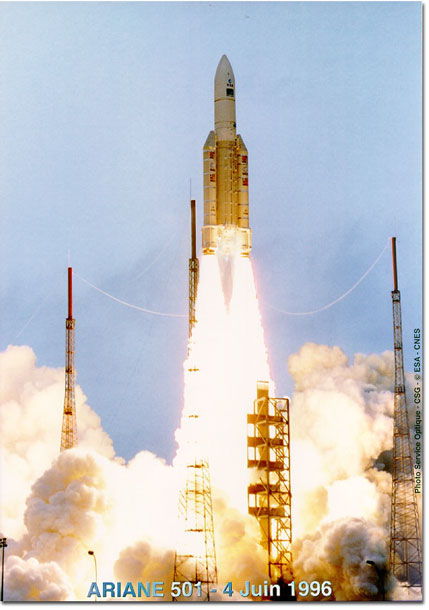
\includegraphics[width=0.9\linewidth]{009_ArianeDecollage.jpg} % Adjust width as needed
	\end{minipage}\hfill
	\begin{minipage}{0.24\textwidth}
		\centering
		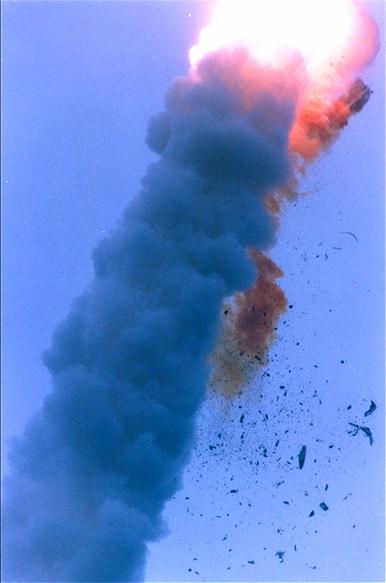
\includegraphics[width=0.9\linewidth]{010_ArianeExplosion1.jpg}
	\end{minipage}
	\begin{minipage}{0.5\textwidth}
		\centering
		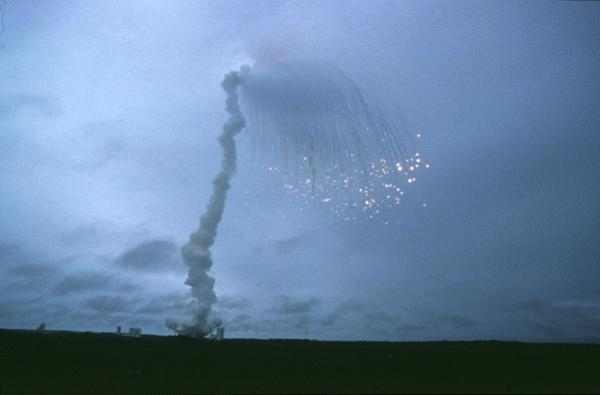
\includegraphics[width=0.9\linewidth]{011_ArianeExplosion3.jpg}
	\end{minipage}
		
	\pagebreak
	
	\section{Encodage des entiers relatifs}
	\subsection{Utilisation d'un bit de signe}
	On sait donc maintenant coder en binaire des entiers positifs -- mais comment faire pour des entiers négatifs (appartenant à l'ensemble des entiers relatifs, noté $\mathbb{Z}$)?
	
	Une première idée consisterait à utiliser ce qu'on appelle un "bit de signe": décider que  lorsqu'on utilise une représentation sur 8 bits pour coder un entier signé, le bit le plus à gauche est dédié au signe du nombre: un "0" indique un nombre positif et un "1" un nombre négatif. De ce fait, seuls les 7 bits restants sont utilisés pour représenter la valeur absolue de l’entier. Ainsi, dans ce système, la plus grande valeur positive que l’on peut représenter n’est pas "11111111" (qui serait interprété comme un nombre négatif à cause du bit de signe à "1"). Au lieu de cela, la plus grande valeur positive possible est "01111111", ce qui correspond à 127 en notation décimale.
	
	\textit{Vocabulaire: on appelle le bit le plus à gauche d'une séquence le "\textbf{bit de poids fort}" et celui le plus à droite le "\textbf{bit de poids faible}" -- correspondant aux puissances de deux plus élevées à gauche qu'à droite.}
	
	Donc, par exemple, 4 sera codé 00000100 et -4 10000100, et si on fait la somme des deux:
	 \[
	\begin{array}{@{}r *{8}{@{\;}c}}
		& 0 & 0 & 0 & 0 & 0 & 1 & 0 & 0 \\
		& 1 & 0 & 0 & 0 & 0 & 1 & 0 & 0 \\
		\cline{2-9}
		& 1 & 0 & 0 & 0 & 1 & 0 & 0 & 0 \\
	\end{array}
	\]
	
	Ce qui, exprimé en décimal, donnerait: 4 + (-4) = -8 -- ce qui est un peu un problème... Face à cette limitation, d'autres méthodes de représentation des nombres négatifs ont été développées pour permettre desopérations arithmétiques plus simples et plus précises.
	
	\subsection{Le complément à 1 -- puis à 2}
	\subsubsection*{Complément à 1}
	Le complément à 1 d'un nombre binaire est le nombre qui change tous les 0 en 1 et tous les 1 en 0.
	Si $n$ est un nombre binaire, le complément à 1 de $n$ est noté \textbf{$\overline{n}$}.
	Par exemple, le complément à 1 de 0011 est 1100.
	
	Donc, par exemple, si fait la somme de 4 (00000100) et de \textbf{$\overline{4}$}, toujours sur 8 bits, on obtient:
	\[
	\begin{array}{@{}r *{8}{@{\;}c}}
		& 0 & 0 & 0 & 0 & 0 & 1 & 0 & 0 \\
		& 1 & 1 & 1 & 1 & 1 & 0 & 1 & 1 \\
		\cline{2-9}
		& 1 & 1 & 1 & 1 & 1 & 1 & 1 & 1 \\
	\end{array}
	\]
	
	Ce n'est évidemment pas ce qu'on cherche -- mais on sent que c'est un début de piste...
	
	\begin{MonExo}[faisons une petite pause Python...]
		Ecrivez, dans IDLE, une fonction CompUn(Lst) qui prend en entrée une liste de bits (par exemple \texttt{[1,0,1,1,0,1]}) et retourne en sortie une liste contenant le complément à 1 (donc "inverse" tous les bits) de la liste en entrée (donc dans le cas précédent: \texttt{[0,1,0,0,1,0]}). Testez votre fonction sur les exemples suivants (la flèche représentant évidemment ce que doit retourner votre fonction):
		\begin{alphenum}
			\item \texttt{CompUn([0])} \textrightarrow  \texttt{[1]}
			\item \texttt{CompUn([1])} \textrightarrow  \texttt{[0]}
			\item \texttt{CompUn([0, 1])} \textrightarrow  \texttt{[1, 0]}
			\item \texttt{CompUn([0,0,1,1,1])} \textrightarrow  \texttt{[1,1,0,0,0]}
		\end{alphenum}
	\end{MonExo}
	\begin{MaReponse}
		\MonPython{003_Comp1.py}
	\end{MaReponse}
	
	\subsubsection*{Complément à 2}
	Ce que l'on va utiliser pour encoder les nombres relatifs est la méthode du \textbf{complément à 2} que l'on peut énoncer de la manière suivante:
	\begin{itemize}
		\item Le bit de poids fort est toujours utilisé pour représenter le signe;
		\item La représentation des nombres positifs est inchangée;
		\item Les nombres négatifs sont le complément à 2 de leur valeur positive:
		\begin{itemize}
			\item On effectue le complément à 1 du nombre;
			\item On ajoute 1.
		\end{itemize} 
	\end{itemize}
	
	Exemples:
	\begin{itemize}
		\item Codage de -3 sur 4 bits:
		\begin{itemize}
			\item $3_{10}$ = $011_2$ (on laisse le bit de poids fort de côté puisqu'il est utilisé pour le signe)
			\item Complément à 1: 100
			\item Complément à 2: 100 + 1 = 101
			\item Donc le codage de -3 est, avec le bit de signe, est le "mot binaire": 1101 
		\end{itemize}
		\item Codage de -4:
		\begin{itemize}
			\item $4_{10}$ = $100_2$ (on laisse le bit de poids fort de côté puisqu'il est utilisé pour le signe)
			\item Complément à 1: 011
			\item Complément à 2: 011 + 1 = 100
			\item Donc le codage de -4 est, avec le bit de signe: 1100
		\end{itemize}
		\item Codage de -1:
		\begin{itemize}
			\item $1_{10}$ = $001_2$
			\item Complément à 1: 110
			\item Complément à 2: 110 + 1 = 111
			\item Donc le codage de -1 est, avec le bit de signe: 1111
		\end{itemize}
	\end{itemize}
	
	Quel est l'intérêt? Essayons de faire quelques sommes de chiffres opposés \textbf{\textit{en ignorant la retenue finale}}:
	\[
	\begin{array}{@{}r *{4}{@{\;}c}}
		& 0 & 0 & 1 & 1 \\
		& 1 & 1 & 0 & 1  \\
		\cline{2-5}
		& 0 & 0 & 0 & 0 \\
	\end{array}
	\]
	\par
	\[
	\begin{array}{@{}r *{4}{@{\;}c}}
		& 0 & 1 & 0 & 0 \\
		& 1 & 1 & 0 & 0  \\
		\cline{2-5}
		& 0 & 0 & 0 & 0 \\
	\end{array}
	\]
	
	\begin{MonExo}[additions d'entiers relatifs]
		En utilisant le complément à deux et toujours sur 4 bits, effectuez les additions binaires suivantes
		\begin{alphenum}
			\item $-1_{10} + 1_{10}$
			\item $2_{10} + -2_{10}$
			\item $1_{10} + -4_{10}$
			\item $-2_{10} + -4_{10}$
			\item $2_{10} + 3_{10}$
		\end{alphenum}
	\end{MonExo}
	\begin{MaReponse}
		\begin{alphenum}
			\item $-1_{10} + 1_{10}$: On vient de voir l'encodage de -1 en complément à 2 donc on peut directement poser l'opération (toujours sur 4 bits):
			\[
			\begin{array}{@{}r *{4}{@{\;}c}}
				& 1 & 1 & 1 & 1 \\
				& 0 & 0 & 0 & 1  \\
				\cline{2-5}
				& 0 & 0 & 0 & 0 \\
			\end{array}
			\]
						
			\item $-2_{10} + -2_{10}$: Codage de -2:
			\begin{itemize}
				\item $2_{10}$ = $010_2$
				\item Complément à 1: 101
				\item Complément à 2: 101 + 1 = 110
				\item Donc le codage de -2 est, avec le bit de signe: 1110
			\end{itemize}
			\[
			\begin{array}{@{}r *{4}{@{\;}c}}
				& 1 & 1 & 1 & 0 \\
				& 0 & 0 & 1 & 0  \\
				\cline{2-5}
				& 0 & 0 & 0 & 0 \\
			\end{array}
			\]
			\item $1_{10} + -4_{10}$: On a déjà l'encodage de -4 en complément à 2 donc on peut directement poser l'opération:
			\[
			\begin{array}{@{}r *{4}{@{\;}c}}
				& 0 & 0 & 0 & 1 \\
				& 1 & 1 & 0 & 0  \\
				\cline{2-5}
				& 1 & 1 & 0 & 1 \\
			\end{array}
			\]
			Ce qui, on le verra dans le tableau plus bas, est bien le mot binaire correspondant à la valeur décimale $-3$.
			\item $-2_{10} + -4_{10}$:
			\[
			\begin{array}{@{}r *{4}{@{\;}c}}
				& 1 & 1 & 1 & 0 \\
				& 1 & 1 & 0 & 0  \\
				\cline{2-5}
				& 1 & 0 & 1 & 0 \\
			\end{array}
			\]
			Ce qui, toujours en vérifiant dans le tableau plus bas, correspond bien à la valeur décimale $-6$.
			\item $2_{10} + 3_{10}$:
			\[
			\begin{array}{@{}r *{4}{@{\;}c}}
				& 0 & 0 & 1 & 0 \\
				& 0 & 0 & 1 & 1  \\
				\cline{2-5}
				& 0 & 1 & 0 & 1 \\
			\end{array}
			\]
			
		(ce qui correspond bien à $+5$ -- juste pour confirmer que les additions d'entiers positifs fonctionnent toujours bien)
		
		\begin{MonAmp}{Important}
			On notera bien que dans la totalité des exemples précédents où on terminait l'addition avec une retenue (donc dans les cas où la somme "réelle" des deux binaires donnait un résultat $> 1111_2$) on ignorait cette retenue - en d'autres termes on ne considérait que les 4 bits les plus à droite (donc de poids le plus faible) pour obtenir le résultat. Ces exemples étaient le a), le b), et le d). On peut aisément vérifier qu'il s'agit des exemples où soit on additionne deux valeurs négatives, soit on additionne une valeur positive à une négative de valeur absolue égale ou inférieure.
		\end{MonAmp}
		 
		\end{alphenum}
	\end{MaReponse}
	
	On constate qu'avec cet encodage, pour tous mots binaires $m_1$ et $m_2$, on peut les additionner en effectuant simplement une addition binaire sans se soucier de leur signe et on obtiendra bien le résultat voulu si on ignore une éventuelle retenue finale.
	
	En appliquant la méthode du complément à 2 encodons sur 4 bits le plus possible d'entiers relatifs -- on obtient:
	\begin{center}	
		\begin{tabular}{|c|c|c|c|>{\centering\arraybackslash}p{2.9cm}|}
			\hline
			\multicolumn{4}{|c|}{\textbf{Mot Binaire}} & \textbf{Entier Relatif}\\ % Merged cells
			\hline
			0 & 0 & 0 & 0 & \parbox{2.9cm}{\centering 0} \\ \hline
			0 & 0 & 0 & 1 & \parbox{2.9cm}{\centering 1} \\ \hline
			0 & 0 & 1 & 0 & \parbox{2.9cm}{\centering 2} \\ \hline
			0 & 0 & 1 & 1 & \parbox{2.9cm}{\centering 3} \\ \hline
			0 & 1 & 0 & 0 & \parbox{2.9cm}{\centering 4} \\ \hline
			0 & 1 & 0 & 1 & \parbox{2.9cm}{\centering 5} \\ \hline
			0 & 1 & 1 & 0 & \parbox{2.9cm}{\centering 6} \\ \hline
			0 & 1 & 1 & 1 & \parbox{2.9cm}{\centering 7} \\ \hline
			1 & 0 & 0 & 0 & \parbox{2.9cm}{\centering -8} \\ \hline
			1 & 0 & 0 & 1 & \parbox{2.9cm}{\centering -7} \\ \hline
			1 & 0 & 1 & 0 & \parbox{2.9cm}{\centering -6} \\ \hline
			1 & 0 & 1 & 1 & \parbox{2.9cm}{\centering -5} \\ \hline
			1 & 1 & 0 & 0 & \parbox{2.9cm}{\centering -4} \\ \hline
			1 & 1 & 0 & 1 & \parbox{2.9cm}{\centering -3} \\ \hline
			1 & 1 & 1 & 0 & \parbox{2.9cm}{\centering -2} \\ \hline
			1 & 1 & 1 & 1 & \parbox{2.9cm}{\centering -1} \\ \hline
		\end{tabular}
	\end{center}
	
	On constate qu'on a représenté ici, sur 4 bits, les entiers allant de -8 à +7; soit les entiers allant de $-(2^3)$ à $(2^3-1)$. On peut facilement se convaincre que cette formule est généralisable en disant que sur \textit{k} bits, on peut représenter des valeurs d'entiers relatifs allant de $-(2^{k-1})$ à $(2^{k-1}-1)$ --- le complément à 2 de l'entier 0 servant à représenter l'entier $-(2^{k-1})$.

	\subsubsection*{Réciproque: passer d'une représentation binaire à l'entier relatif}
	
	Pour convertir un nombre binaire stocké sur un octet en complément à deux vers sa représentation en entier relatif, suivez les étapes suivantes:
	\begin{enumerate}
		\item Si le bit le plus à gauche (bit de signe) est 0, le nombre est positif -- il suffit de  convertir les 7 bits restants directement de base 2 à base 10.
		\item Sinon, le nombre est négatif:
		\begin{enumerate}
			\item Inversez tous les bits.
			\item Ajoutez 1 au résultat.
			\item Convertissez les 7 bits restants en base 10 et ajoutez un signe négatif devant le résultat.
		\end{enumerate}
	\end{enumerate}
	
	\begin{MonExo}[conversions en décimal]
		Convertissez en décimal les nombres représentés en utilisant la méthode du complément à deux suivant
		\begin{alphenum}
			\item 00001000
			\item 11111101
			\item 11111000
		\end{alphenum}
	\end{MonExo}
	\begin{MaReponse}
		\begin{alphenum}
			\item 00001000: le bit de poids fort (le plus à gauche) est 0, donc c'est un entier positif, donc on convertit directement de binaire à décimal: en l'occurence on voit que ce nombre est égal à $2^3$ soit 8.
			\item 11111101: cette fois, le nombre est négatif:
			\begin{itemize}
				\item Inversion des bits / complément à 1: 00000010
				\item Ajout de 1: 00000011
				\item Conversion en base 10: $11_2 = 3_{10}$
				\item Ajout du signe moins -- le résultat est: $-3$.
			\end{itemize}
			Note: pour vous en convaincre, vous pouvez poser l'addition 11111101 + 000000011 et vérifier que vous retombez bien sur 0 (en ignorant bien sûr la retenue finale).
			\item 11111000: même démarche:
			\begin{itemize}
				\item Inversion des bits / complément à 1: 00000111
				\item Ajout de 1: 00001000
				\item Conversion en base 10: $1000_2 = 8_{10}$
				\item Ajout du signe moins -- le résultat est: $-8$.
			\end{itemize}
		\end{alphenum}
	\end{MaReponse}
	
	\pagebreak
	
	\section{Représentation approximative des nombres réels}
	\begin{MonAmp}{ATTENTION}
		Ce chapitre est assez complexe, notamment au niveau calculatoire. Il est important que vous en compreniez les concepts et les modes de calcul, mais \textbf{\uline{il ne vous sera pas demandé de connaître précisément la norme IEEE 754 -- c'est hors programme}}. C'est une des raisons pour lesquelles ce chapitre contient relativement moins d'exercices que les autres.
	\end{MonAmp}
	
	\vspace{0.5\baselineskip}
	
	\begin{MonExo}[commençons par essayer de voir le problème]
		Dans une console Python, effectuez les calculs suivants:
		\begin{alphenum}
			\item \texttt{0.5 - 0.2 - 0.2 - 0.1}
			\item \texttt{9007199254740992.0 + 2.0}
			\item \texttt{9007199254740992.0 + 1.0 + 1.0}
			\item \texttt{1.0 + 1.0 + 9007199254740992.0}
		\end{alphenum}
	\end{MonExo}
	\begin{MaReponse}
		L'exécution des commandes ci-dessus en console Python donnent le résultat suivant:
		\par
			\begin{minipage}{0.95\textwidth}
			\centering
			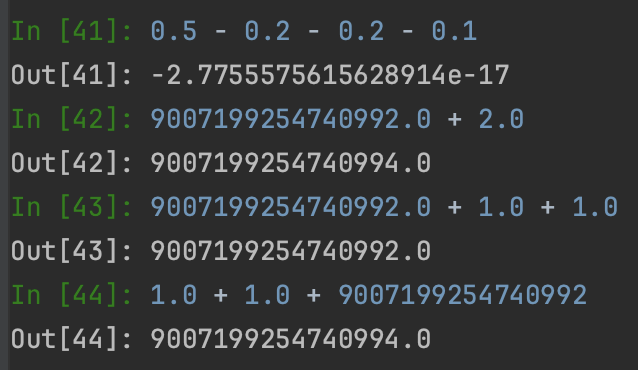
\includegraphics[width=0.5\linewidth]{012_FloatPython.png}
		\end{minipage}
		\par
		Je pense que les erreurs et incohérences sautent aux yeux...
	\end{MaReponse}
	
	La raison de ces erreurs est qu'il n'est pas possible de représenter la totalité des nombres réels (de l'ensemble mathématique $\mathbb{R}$) avec exactitude en binaire -- ce qui en première analyse se comprend intuitivement très bien en constatant que le nombre de réels compris entre 0 et 1 est infini, tandis que le nombre de combinaisons de bits sur une taille mémoire donnée est nécessairement finie. On doit donc recourir à des approximations -- et l'objet de ce chapitre est de comprendre comment ces approximations fonctionnent.
	
	\subsection{Puissances négatives de 2}
	Jusqu'à présent, nous avons travaillé avec des puissances successives de deux toujours positives -- 1, 2, 4, 8, 16, 32, etc... -- et en avons considéré la somme pour convertir des nombres de la base 2 à la base 10 -- par exemple:
	\begin{tabbing}
		$10_{10}$ \==  $(8 + 2)_{10}$ \\
		\>= $(1 \times 2^{3} + 0 \times 2^{2} + 1 \times 2^{1} + 0 \times 2^{0})_{10}$ \\
		\>= $(1010)_{2}$
	\end{tabbing}
	
	Nous allons ici étendre cette notion aux puissances \textit{négatives} de 2 pour représenter des nombres compris dans l'intervalle [0, 1[:
	 \[
	\begin{array}{|c|c|c|c|c|c|}
		\hline
		2^{-1} & 2^{-2} & 2^{-3} & 2^{-4} &  2^{-5} & \ldots \\
		\hline
		0.5 & 0.25 & 0.125 & 0.0625 & 0.03125 &  \ldots \\
		\hline
	\end{array}
	\]
	
	Ainsi, en utilisant cette notation, le mot binaire 1010 codé sur 4 bits aura pour valeur:
		 \[
	\begin{array}{|c|c|c|c|}
		\hline
		2^{-1} & 2^{-2} & 2^{-3} & 2^{-4} \\
		\hline
		1 & 0 & 1 & 0  \\
		\hline
	\end{array}
	\]
	
	Que l'on va calculer ainsi:
	
	\begin{tabbing}
		$1010_{2}$ \==  $(1 \times 2^{-1} + 0 \times 2^{-2} + 1 \times 2^{-3} + 0 \times 2^{-4})_{10}$ \\
		\>= $(0,5 + 0,125)_{10}$ \\
		\>= $(0,625)_{2}$
	\end{tabbing}
	
	\subsection{La notation scientifique}
	On utilise beaucoup, en mathématiques et en sciences, ce qu'on appelle la \textit{notation scientifique} des nombres décimaux. Celle-ci se compose d'un signe (+ ou -); d'une \textit{mantisse}, notée $m$ et comprise dans l'intervalle [1, 10[; et d'un \textit{exposant}, nombre entier relatif noté $n$. L'écriture de cette valeur est alors $\pm m \times 10^n$. Ainsi, spécifiquement:
	
	\[
	\begin{array}{rll}
		2\ 156 & \text{s'écrit } & +2,156 \times 10^3 \\
		-398\ 879,62 & \text{s'écrit } & -3,9887962 \times 10^5 \\
		0,000142 & \text{s'écrit } & +1,42 \times 10^{-4} \\
		1,34 & \text{s'écrit } & +1,34 \times 10^0 \\
	\end{array}
	\]
	
	\subsection{La norme IEEE 754}
	Cette norme, développée dans les années 1980 aux USA, existe en deux versions, l'une, dite "codage simple précision", pour une représentation sur 32 bits (4 octets), et l'autre, dite "codage double précision", pour une représentation sur 64 bits (8 octets). Dans les deux cas elle s'appuie sur le même principe que la notation scientifique -- à s'avoir une décomposition du nombre en une somme de puissances, utilise les puissances négatives de 2 pour décrire le plus précisément possible la mantisse, et s'écrit sous la forme suivante:
	
	\[(-1)^s\cdot (1+m) \times 2^{(n-d)}\]
	
	\begin{itemize}
		\item $s$ est le bit de signe, valant 0 ou 1;
		\item $m$ est la mantisse, comprise (puisqu'on raisonne ici non plus en base 10 mais en base 2) dans l'intervalle [0, 1[;
		\item $n$ est toujours l'exposant, mais il est cette fois "\textit{décalé}" (on peut également dire "\textit{biaisé}") d'une valeur d qui dépend du format choisi (32 ou 64 bits).
	\end{itemize}
	
	Ecrite de la sorte en mémoire et encodée sur 32 bits, la valeur d'un nombre flottant sera structurée comme suit:
	
	 \[ \overbrace{\underbrace{\text{ Signe }}_{s}}^{\text(1\ bit)} \quad \overbrace{\underbrace{\text{ Exposant }}_{n}}^{\text(8\  bits)} \quad \overbrace{\underbrace{\text{ Mantisse }}_{m}}^{\text(23\  bits)} \]
	
	Voyons un exemple concret, le mot $M$ de 32 bits suivant:
	\begin{center}
		11000011010101101100000000000000
	\end{center}
	Commençons par le décomposer en signe (bit de poids fort), exposant (8 bits suivants), et mantisse (23 bits restants):
	\[ \overbrace{1}^{\text signe} \quad
	\overbrace{10000110}^{\text exposant} \quad
	\overbrace{10101101100000000000000}^{\text mantisse} \]
	
	Calculons alors sa valeur décimale:
	\[
	\begin{array}{lll}
		\text{signe} & \text{=} & -1^1\\
		& \text{=} & -1\\
		\\
		\text{exposant} & \text{=} & 2^7 + 2^2 + 2^1\\
		& \text{=} & 128 + 4 + 2\\
		& \text{=} & 134\\
		\\
		\text{mantisse} & \text{=} & 2^{-1} + 2^{-3} + 2^{-5} + 2^{-6} + 2^{-8} + 2^{-9}\\
		& \text{=} & 0,677734375\\
	\end{array}
	\]
	
	Appliquons à présent la formule générale décrite plus haut ($(-1)^s\cdot (1+m) \times 2^{(n-d)}$) en utilisant un décalage $d$ de 127 puisque nous étudions un encodage sur 32 bits:
	\[
	\begin{array}{lll}
		M& \text{=} & -1 \times (1+0,677734375) \times 2^{(134 - 127)}\\
		& \text{=} & -1,677734375 \times 2^7\\
		& \text{=} & -214,75\
	\end{array}
	\]
		
		\begin{MonExo}[Entrainons-nous...]
		Convertissons quelques réels codés sur 32 bits pour s'entrainer...
		\begin{alphenum}
			\item
				\begin{tabular}{|c|c|c|c|c|c|c|c|c|c|c|c|c|c|c|c|} % One 'c' column type for each letter in the word
					\hline
					0&1&0&0&0&0&0&0&1&1&0&1&0&1&0&0 \\
					\hline
					0&0&0&0&0&0&0&0&0&0&0&0&0&0&0&0 \\
					\hline
				\end{tabular}
			\item
				\begin{tabular}{|c|c|c|c|c|c|c|c|c|c|c|c|c|c|c|c|} % One 'c' column type for each letter in the word
					\hline
					1&0&1&1&1&1&1&0&1&1&1&1&1&0&0&0 \\
					\hline
					0&0&0&0&0&0&0&0&0&0&0&0&0&0&0&0 \\
					\hline
				\end{tabular}
		\end{alphenum}
	\end{MonExo}
	\begin{MaReponse}
		\begin{alphenum}
			\item
			\begin{tabular}{|c|c|c|c|c|c|c|c|c|c|c|c|c|c|c|c|} % One 'c' column type for each letter in the word
				\hline
				0&1&0&0&0&0&0&0&1&1&0&1&0&1&0&0 \\
				\hline
				0&0&0&0&0&0&0&0&0&0&0&0&0&0&0&0 \\
				\hline
			\end{tabular}
			\par
			Isolons tout d'abord les différentes composantes de ce mot binaire:
			\begin{itemize}
				\item Signe: 0
				\item Exposant: 10000001
				\item Mantisse: 10101000000000000000000
			\end{itemize}
			Comme ci-dessus, calculons à présent les valeurs de ces différentes composantes:
			\[
			\begin{array}{lll}
				\text{signe} & \text{=} & -1^0\\
				& \text{=} & +1\\
				\\
				\text{exposant} & \text{=} & 2^7 + 2^0\\
				& \text{=} & 128 + 1\\
				& \text{=} & 129\\
				\\
				\text{mantisse} & \text{=} & 2^{-1} + 2^{-3} + 2^{-5}\\
				& \text{=} & 0,65625\\
			\end{array}
			\]
			Appliquons enfin la formule générale décrite plus haut ($(-1)^s\cdot (1+m) \times 2^{(n-d)}$) en utilisant un décalage $d$ de 127 puisque nous étudions un encodage sur 32 bits:
			\[
			\begin{array}{lll}
				M& \text{=} & 1 \times (1+0,65625) \times 2^{(129 - 127)}\\
				& \text{=} & 1,65625 \times 2^2\\
				& \text{=} & 6,625\
			\end{array}
			\]
			
			\item
			\begin{tabular}{|c|c|c|c|c|c|c|c|c|c|c|c|c|c|c|c|} % One 'c' column type for each letter in the word
				\hline
				1&0&1&1&1&1&1&0&1&1&1&1&1&0&0&0 \\
				\hline
				0&0&0&0&0&0&0&0&0&0&0&0&0&0&0&0 \\
				\hline
			\end{tabular}
			\par
			Isolons tout d'abord les différentes composantes de ce mot binaire:
			\begin{itemize}
				\item Signe: 1
				\item Exposant: 01111101
				\item Mantisse: 11110000000000000000000
			\end{itemize}
			Comme ci-dessus, calculons à présent les valeurs de ces différentes composantes:
			\[
			\begin{array}{lll}
				\text{signe} & \text{=} & -1^1\\
				& \text{=} & -1\\
				\\
				\text{exposant} & \text{=} & 2^6 + 2^5 + 2^4 + 2^3 + 2^2 + 2^0 \\
				& \text{=} & 64 + 32 + 16 + 8 + 4 + 1\\
				& \text{=} & 125\\
				\\
				\text{mantisse} & \text{=} & 2^{-1} + 2^{-2} + 2^{-3} + 2^{-4}\\
				& \text{=} & 0,9375\\
			\end{array}
			\]
			Appliquons enfin la formule générale décrite plus haut ($(-1)^s\cdot (1+m) \times 2^{(n-d)}$) en utilisant un décalage $d$ de 127 puisque nous étudions un encodage sur 32 bits:
			\[
			\begin{array}{lll}
				M& \text{=} & -1 \times (1+0,9375) \times 2^{(125 - 127)}\\
				& \text{=} & -1,9375 \times 2^{-2}\\
				& \text{=} & -1,9375 \times 0,25\\
				& \text{=} & -0,484375\
			\end{array}
			\]
		\end{alphenum}
	\end{MaReponse}
	
	\begin{MonExo}[C'est un peu fastidieux... et si on codait ça?]
		\begin{alphenum}
			\item Sur papier, écrire en pseudo-code l'algorithme d'une fonction qui prend en entrée une liste de 32 éléments représentant les 32 bits encodant un nombre flottant et qui calcule puis renvoie la valeur décimal du réel correspondant.
			\item Dans IDLE, écrire cette fonction en Python. Si vous avez terminé, rendez cette fonction robuste -- qu'elle sache gérer des listes n'ayant pas le bon nombre d'éléments, ou ne contenant pas que des 0 ou des 1 (utilisez la fonction \texttt{assert} notamment)...
		\end{alphenum}
	\end{MonExo}
	\begin{MaReponse}
		\begin{algorithmic}[1]
			\Require{$Lst$, liste de 32 bits ($\in \{0,1\}$)}
			\Ensure{$res \in \mathds{R}$}
			\Function{ConvBinEnReel}{Lst}
			\State exposant $\leftarrow$ 0
			\State mantisse $\leftarrow$ 0.0
			\Comment{C'est un nb réel $\in [0,1[}$
			\\
			\State signe $\leftarrow$ $-1^{Lst([0])}$
			\Comment{Calcul signe sur le 1\textsuperscript{er}  elt de la liste d'entrée}
			\\
			\For{$i=1$ à $8$}
			\Comment{Calcul exposant sur les 8 elts suivants}
			\State{puiss $\leftarrow 8-i$}
			\Comment{indice 1  $\leftrightarrow 2^7$; $i=2 \leftrightarrow 2^6$; ...;  $i=8 \leftrightarrow 2^0$}
			\If{$Lst[i]=1$}
			\State{exposant $\leftarrow exposant + 2^{puiss}$}
			\EndIf
			\EndFor
			\State{exposant $\leftarrow exposant -127$}
			\Comment{Application du décalage sur 32 bits}
			\\
			\For{$i=9$ à $31$}
			\Comment{Calcul mantisse sur les 23 derniers elts}
			\State{puiss $\leftarrow 8-i$}
			\Comment{indice 9  $\leftrightarrow 2^{-1}$; $i=10 \leftrightarrow 2^{-2}$; ...;  $i=31 \leftrightarrow 2^{-23}$}
			\If{$Lst[i]=1$}
			\State{mantisse $\leftarrow mantisse + 2^{puiss}$}
			\EndIf
			\EndFor
			\State{mantisse $\leftarrow 1 + mantisse$}
			\Comment{Application du "(1+m)" de la formule}
			\\
			\State{resultat $\leftarrow signe \times mantisse \times exposant$}
			\\
			\State\Return{resultat}
			\EndFunction
		\end{algorithmic}
		
		\MonPython{004_ConvBin2Float.py}
	\end{MaReponse}
	
	\subsection{Alors d'où viennent les erreurs qu'on a vues?}
	Le problème est qu'il n'est en général pas possible de coder \textit{exactement} un nombre réel avec ce système -- sauf si, par chance, il peut se décomposer exactement de cette manière. L'ordinateur en est donc réduit à stocker des approximations des valeurs qu'on lui donne.
	
	Par exemple: le nombre flottant le plus proche de 1,2 est
	\begin{center}
		0 -- 01111111 -- 00110011001100110011001
	\end{center}
	La valeur exacte de ce nombre, si on le développe comme on l'a fait plus tôt, est de 1.2000000476837158 -- ce qui est évidemment une différence négligeable pour la représentation de valeurs à l'échelle humaine (qu'il s'agisse, de distances, de pourcentages dans des contextes divers, de montants d'argent, de mesures physiques telles que le poids ou la vitesse d'un objet...). Cependant, il faut bien avoir conscience de l'existence de ces approximations.
	
	Deux remarques:
	\begin{itemize}
		\item Il est évident ici que l'ordinateur utilise une méthode d'arrondis pour passer d'un mot binaire à sa valeur décimale et réciproquement. Cette méthode est hors programme.
		\item Si cependant c'est un sujet qui vous intéresse n'hésitez pas à consulter  \href{https://www.h-schmidt.net/FloatConverter/IEEE754.html}{ce site} pour voir plus en détails comment différentes valeurs réelles sont effectivement codées au moyen de la norme IEEE 754.
	\end{itemize}
	
	
	En tout état de cause, l'objet de ce chapitre est principalement de vous alerter sur deux points fondamentaux:
	
	\begin{itemize}
		\item Le fait \textbf{qu'il ne faut jamais} effectuer des tests d'égalité entre nombres flottants dans un programme (on l'a vu en début de chapitre, et on en avait vu également des exemples dans le cours sur Python);
		\item Le fait que dans des contextes où les besoins de précision sont hors du commun (dans certaines disciplines scientifiques par exemple), il sera nécessaire de trouver des moyens de contourner ces difficultés pour éviter de générer de réelles erreurs.
	\end{itemize}
	
	\pagebreak
	
	\section{Représentation des caractères}
	
	\begin{MonAmp}{ATTENTION}
		Comme le chapitre précédent, celui-ci a pour vocation d'être une introduction au codage des caractères -- vous devez en comprendre les principes et les mécanismes, mais \textbf{\uline{il ne vous sera pas demandé de connaître précisément le normes d'encodage (ASCII et Unicode) -- c'est hors programme}}. 	\end{MonAmp}
	
	\subsection{Code ASCII}
	
	Les ordinateurs ne stockent que des 0 et des 1; on sait assez simplement établir une correspondance entre un nombre décimal et sa traduction en binaire. Partant de ces deux constats, on a initialement établi une correspondance unique entre chaque caractère et un entier naturel -- on appelle cette démarche le \textit{charset}.
	
	Ceci a donné naissance en 1963 au code ASCII (\textit{American Standard Code for Information Interchange}), toujours en usage, et permettant d'encoder 128 caractères: 33 caractères dits de contrôle (codes 0 à 32 et code 127 -- ils incluent des caractères "blancs" comme les espaces ou les tabulations, des suppressions, des retours à la ligne, des marqueurs de début et de fin de texte...), 94 caractères standards (codes 33 à 126) comportant les 26 lettres minuscules, les 26 lettres majuscules, les 10 chiffres, et 32 symboles (ponctuation, symboles arithmétiques...).
	
	Le tableau ci-dessous vous présente tout ceci exhaustivement (pour votre culture générale -- il est évident \textbf{que ce n'est pas à connaitre par cœur!}). La colonne code contient deux valeurs - d'abord en décimal, puis en hexadécimal.
	
	\begin{center}
			\begin{tabular}{|c|l||c|l||c|l||c|l|}
			\hline
			Code & Car. & Code & Car. & Code & Car. & Code & Car.  \\
			\hline
			0, 0 & NUL & 32, 20 & Espace & 64, 40 & @ & 96, 60 & ` \\
			1, 1 & SOH & 33, 21 & ! & 65, 41 & A & 97, 61 & a \\
			2, 2 & STX & 34, 22 & " & 66, 42 & B & 98, 62 & b \\
			3, 3 & ETX & 35, 23 & \# & 67, 43 & C & 99, 63 & c \\
			4, 4 & EOT & 36, 24 & \$ & 68, 44 & D & 100, 64 & d \\
			5, 5 & ENQ & 37, 25 & \% & 69, 45 & E & 101, 65 & e \\
			6, 6 & ACK & 38, 26 & \& & 70, 46 & F & 102, 66 & f \\
			7, 7 & BEL & 39, 27 & ' & 71, 47 & G & 103, 67 & g \\
			8, 8 & BS & 40, 28 & ( & 72, 48 & H & 104, 68 & h \\
			9, 9 & HT & 41, 29 & ) & 73, 49 & I, 49 & 105, 69 & i \\
			10, A & LF & 42, 2A & * & 74, 4A & J & 106, 6A & j \\
			11, B & VT & 43, 2B & + & 75, 4B & K & 107, 6B & k \\
			12, C & FF & 44, 2C & , & 76, 4C & L & 108, 6C & l \\
			13, D & CR & 45, 2D & - & 77, 4D & M & 109, 6D & m \\
			14, E & SO & 46, 2E & . & 78, 'E & N & 110, 6E & n \\
			15, F & SI & 47, 2F & / & 79, 4F & O & 111, 6F & o \\
			16, 10 & DLE & 48, 30 & 0 & 80, 50 & P & 112, 70 & p \\
			17, 11 & DC1 & 49, 31 & 1 & 81, 51 & Q & 113, 71 & q \\
			18, 12 & DC2 & 50, 32 & 2 & 82, 52 & R & 114, 72 & r \\
			19, 13 & DC3 & 51, 33 & 3 & 83, 53 & S & 115, 73 & s \\
			20, 14 & DC4 & 52, 34 & 4 & 84, 54 & T & 116, 74 & t \\
			21, 15 & NAK & 53, 35 & 5 & 85, 55 & U & 117, 75 & u \\
			22, 16 & SYN & 54, 36 & 6 & 86, 56 & V & 118, 76 & v \\
			23, 17 & ETB & 55, 37 & 7 & 87, 57 & W & 119, 77 & w \\
			24, 18 & CAN & 56, 38 & 8 & 88, 58 & X & 120, 78 & x \\
			25, 19 & EM & 57, 39 & 9 & 89, 59 & Y & 121, 79 & y \\
			26, 1A & SUB & 58, 3A & : & 90, 5A & Z & 122, 7A & z \\
			27, 1B & ESC & 59, 3B & ; & 91, 5B & [ & 123, 7B & \{ \\
			28, 1C & FS & 60, 3C & < & 92, 5C & \textbackslash & 124, 7C & | \\
			29, 1D & GS & 61, 3D & = & 93, 5D & ] & 125, 7D & \} \\
			30, 1E & RS & 62, 3E & > & 94, 5E & \textasciicircum & 126, 7E & \textasciitilde \\
			31, 1F & US & 63, 3F & ? & 95, 5F & \_ & 127, 7F & DEL \\
			\hline
		\end{tabular}
	\end{center}
	
	Un texte codé en ASCII est  simplement une suite d'octets (on va voir pourquoi tout de suite) correspondant à la séquence de caractères et utilisant les valeurs du tableau ci-dessus. Par exemple la phrase \texttt{Bonjour le monde!} correspond à la séquence d'octets:
	
	\ttfamily
	\begin{center}
		\begin{tabular}{|c|c|c|c|c|c|c|c|c|c|c|c|c|c|c|c|c|}
			\hline
			B&o&n&j&o&u&r& &l&e& &m&o&n&d&e&! \\
			\hline
			42&6F&6E&6A&6F&75&72&20&6C&65&20&6D&6F&6E&64&65&21 \\
			\hline
		\end{tabular}
	\end{center}
	
	\normalfont
	\MaQuestion{Ce tableau nous permet donc d'encoder des textes simples, mais il est loin d'être parfait. A première vue, qu'est-ce qui ne va pas? Quel(s) problème(s) va-t-on rapidement rencontrer?}
	\begin{MaReponse}
		Il manque énormément de caractères -- et d'autant plus si on n'est pas anglophone! Déjà, pour les francophones, on note qu'il n'y a aucun accent. Mais que devaient penser les Arabes, les Chinois, les Russes...?
	\end{MaReponse}
	
		\MaQuestion{Sur combien de bits va-t-on encoder ces caractères ASCII?}
	\begin{MaReponse}
		On compte 128 caractères soit (et ce n'est évidemment pas un hasard) $2^7$. Il serait donc possible de n'utiliser que 7 bits pour coder les caractères ASCII.
		
		En pratique, on a toujours codé ces caractères sur un octet (donc 8 bits) en utilisant à l'origine le bit de poids fort comme un mécanisme de contrôle d'erreur (qui étaient fréquentes avec les premières mémoires électroniques). Le principe était d'en faire un bit de parité: il était positionné à 0 ou à 1 de manière à ce que tous les caractères aient toujours un nombre pair de bits à 1; et si ce n'était pas le cas, une erreur était détectée.
	\end{MaReponse}
	
	\subsection{Normes ISO 8859}
	
	Partant du constat de ces faiblesses, on a progressivement amélioré les capacités et méthodes de codage de texte pour les enrichir et les rendre compatibles avec de plus en plus de langues et de caractères spéciaux:
	\begin{itemize}
		\item On a commencé par utiliser ce fameux 8\textsuperscript{ème} bit de l'octet pour \textit{doubler} le nombre de caractères qu'on pouvait coder (norme ISO 8859) et arriver à 256, les 128 premiers demeurant les caractères ASCII. On a appelé cette nouvelle norme "ANSI".
		\item C'était bien mieux, mais encore insuffisant -- pensez encore une fois aux Russes, Arabes, et Chinois pour ne citer qu'eux. On a donc multiplié ces codages en créant des \textit{pages} (ou tables de correspondances) de codes pour différents contextes, numérotées et nommées "8859-\textit{n}". Pour chaque page, on conserve les caractères ASCII sur les 128 premiers codes et on utilise les 128 restants pour coder des caractères spécifiques à une zone géographique. Ainsi (quelques exemples):
		\begin{itemize}
			\item La page 8859-1 est spécifique aux caractères de l'Europe occidentale;
			\item La page 8859-5 est spécifique aux caractères cyriliques (donc, entre autres, au Russe);
			\item La page 8859-6 est spécifique à l'Arabe;
			\item La page 8859-9 est spécifique au Turc et au Kurde;
			\item etc...
		\end{itemize} 
	\end{itemize}
	
	Tout ceci constitue évidemment une amélioration (16 tables ont été développées en tout, avec donc une capacité d'encodage totale 17 fois supérieure à ce que permettait la seule norme ASCII) mais:
	
	\begin{itemize}
		\item Ca reste largement insuffisant: 10 de ces 16 pages sont consacrées aux seules langues latines!
		\item Le fonctionnement impose de spécifier avant tout texte quelle page d'encodage on utilise (puisqu'un même caractère peut être codé différemment suivant la norme utilisée) et de s'y tenir -- ce qui peut entraîner beaucoup de confusion. Avez-vous par exemple déjà croisé un mail ou une page web ressemblant à ceci?
	\end{itemize}
	\begin{minipage}{0.95\textwidth}
		\centering
		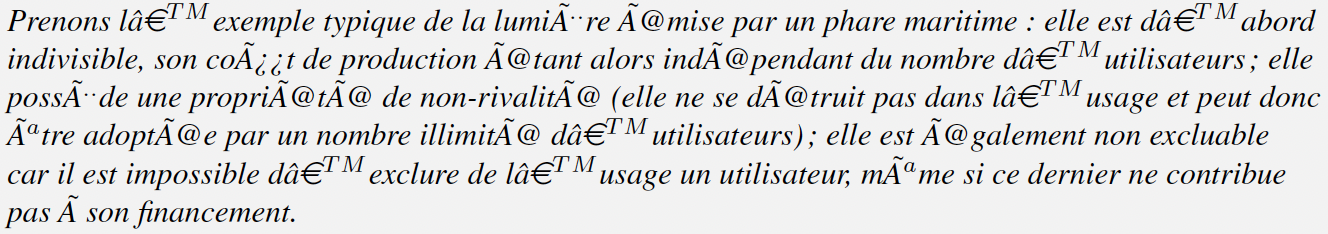
\includegraphics[width=0.95\linewidth]{013_ANSI.png}
	\end{minipage}
	
	\subsection{Une petite pause Python...}
	Avant de passer à la norme Unicode qui est le coeur de ce chapitre, faisons un petit détour par Python, et plus spécifiquement:
	\begin{itemize}
		\item Quelques éléments de manipulation de chaines de caractères que nous n'avons pas encore vus jusqu'à présent;
		\item Quelques fonctions spécifiques que propose le langage pour aller d'un caractère à son code et réciproquement.
	\end{itemize}
	
	Jusqu'à présent on n'a pas vraiment manipulé de chaines de caractères -- on a affiché des messages à l'écran qui en utilisaient ("\texttt{print('Le nombre est pair'})" par exemple), ou, par le biais de la fonction \texttt{input}, on a pris du texte saisi par l'utilisateur en entrée. Mais on ne s'est pas vraiment demandé \textit{ce qu'était} une variable de type "string".
	
	
	
	\subsection{La norme Unicode}
	\pagebreak
	\section{Circuits \& logique booléenne}
	
\end{document}
%Eléments manquants:
